%% abtex2-modelo-trabalho-academico.tex, v-1.9.7 laurocesar
%% Copyright 2012-2018 by abnTeX2 group at http://www.abntex.net.br/ 
%%
%% This work may be distributed and/or modified under the
%% conditions of the LaTeX Project Public License, either version 1.3
%% of this license or (at your option) any later version.
%% The latest version of this license is in
%%   http://www.latex-project.org/lppl.txt
%% and version 1.3 or later is part of all distributions of LaTeX
%% version 2005/12/01 or later.
%%
%% This work has the LPPL maintenance status `maintained'.
	%% 
%% The Current Maintainer of this work is the abnTeX2 team, led
%% by Lauro César Araujo. Further information are available on 
%% http://www.abntex.net.br/
%%
%% This work consists of the files abntex2-modelo-trabalho-academico.tex,
%% abntex2-modelo-include-comandos and abntex2-modelo-references.bib
%%

% ------------------------------------------------------------------------
% ------------------------------------------------------------------------
% abnTeX2: Modelo de Trabalho Academico (tese de doutorado, dissertacao de
% mestrado e trabalhos monograficos em geral) em conformidade com 
% ABNT NBR 14724:2011: Informacao e documentacao - Trabalhos academicos -
% Apresentacao
% ------------------------------------------------------------------------
% ------------------------------------------------------------------------

\documentclass[
  % -- opções da classe memoir --
  12pt,       % tamanho da fonte
  openright,      % capítulos começam em pág ímpar (insere página vazia caso preciso)
  twoside,      % para impressão em recto e verso. Oposto a oneside
  a4paper,      % tamanho do papel. 
  % -- opções da classe abntex2 --
  %chapter=TITLE,   % títulos de capítulos convertidos em letras maiúsculas
  %section=TITLE,   % títulos de seções convertidos em letras maiúsculas
  %subsection=TITLE,  % títulos de subseções convertidos em letras maiúsculas
  %subsubsection=TITLE,% títulos de subsubseções convertidos em letras maiúsculas
  % -- opções do pacote babel --
  english,      % idioma adicional para hifenização
  french,       % idioma adicional para hifenização
  spanish,      % idioma adicional para hifenização
  brazil        % o último idioma é o principal do documento
  ]{abntex2}

% ---
% Pacotes básicos 
% ---
\usepackage{times}      % Usa a fonte Latin Modern      
\usepackage[T1]{fontenc}    % Selecao de codigos de fonte.
\usepackage[utf8]{inputenc}   % Codificacao do documento (conversão automática dos acentos)
\usepackage{indentfirst}    % Indenta o primeiro parágrafo de cada seção.
\usepackage{color}        % Controle das cores
\usepackage{graphicx}     % Inclusão de gráficos
\usepackage{microtype}      % para melhorias de justificação
\usepackage{makecell}
\usepackage{datetime}
\usepackage[brazilian,hyperpageref]{backref}   % Paginas com as citações na bibl
\usepackage[alf]{abntex2cite} % Citações padrão ABNT
\usepackage{xcolor}


\usepackage{newfloat}
\usepackage{verbatim}
\usepackage{listings}
\usepackage{float}


\lstset{
    language=Python,
    basicstyle=\ttfamily\footnotesize,
    keywordstyle=\color{blue},
    commentstyle=\color{gray},
    stringstyle=\color{green},
    numbers=left,
    numberstyle=\tiny\color{black},
    stepnumber=1,
    numbersep=10pt,
    backgroundcolor=\color{white},
    frame=single,
    rulecolor=\color{black},
    captionpos=b,
    breaklines=true,
    showspaces=false,
    showstringspaces=false,
    showtabs=false,
    tabsize=4,
    xleftmargin=1.5em,
    framexleftmargin=1.5em,
    framexbottommargin=5pt,
    framextopmargin=5pt,
    belowskip=0pt % adiciona espaço entre a legenda do quadro e o código
}


\newdateformat{mydate}{\THEDAY\space de \monthname[\THEMONTH], \THEYEAR}
% ---
% Configurações do pacote backref
% Usado sem a opção hyperpageref de backref
\renewcommand{\backrefpagesname}{Citado na(s) página(s):~}
% Texto padrão antes do número das páginas
\renewcommand{\backref}{}
% Define os textos da citação
\renewcommand*{\backrefalt}[4]{
  \ifcase #1 %
    Nenhuma citação no texto.%
  \or
    Citado na página #2.%
  \else
    Citado #1 vezes nas páginas #2.%
  \fi}%
% ---

% ---
% Informações de dados para CAPA e FOLHA DE ROSTO
% ---
\titulo{Representações sociais da poluição segundo os discentes do Novo Ensino Médio}
\autor{João Henrique da Silva}
\local{Maringá}
\data{\today}
\orientador{Prof. Dr. Carlos Alberto de Oliveira Magalhães Júnior}
\instituicao{
  Universidade Estadual de Maringá - UEM
  \par
  Departamento de Ciências - DCI
  \par
  Programa de Pós-Graduação em Rede Nacional para Ensino das \\
  Ciências Ambientais -PROFCIAMB}
\tipotrabalho{Dissertação (Mestrado)}
% O preambulo deve conter o tipo do trabalho, o objetivo, 
% o nome da instituição e a área de concentração 
\preambulo{Projeto de pesquisa acerca das representações sociais da poluição apropriadas pelos discentes do Novo Ensino Médio.}
% ---


% ---
% Configurações de aparência do PDF final

% alterando o aspecto da cor azul
\definecolor{blue}{RGB}{41,5,195}

% informações do PDF
\makeatletter
\hypersetup{
      %pagebackref=true,
    pdftitle={\@title}, 
    pdfauthor={\@author},
      pdfsubject={\imprimirpreambulo},
      pdfcreator={LaTeX with abnTeX2},
    pdfkeywords={abnt}{latex}{abntex}{abntex2}{trabalho acadêmico}, 
    colorlinks=true,          % false: boxed links; true: colored links
      linkcolor=blue,           % color of internal links
      citecolor=blue,           % color of links to bibliography
      filecolor=magenta,          % color of file links
    urlcolor=blue,
    bookmarksdepth=4
}
\makeatother
% --- 

% ---
% Posiciona figuras e tabelas no topo da página quando adicionadas sozinhas
% em um página em branco. Ver https://github.com/abntex/abntex2/issues/170
\makeatletter
\setlength{\@fptop}{5pt} % Set distance from top of page to first float
\makeatother
% ---

\DeclareFloatingEnvironment[
  fileext=loq,
  listname={Lista de quadros},
  name=Quadro,
  placement=tbhp,
]{quadro}


% --- 
% Espaçamentos entre linhas e parágrafos 
% --- 

% O tamanho do parágrafo é dado por:
\setlength{\parindent}{1.3cm}

% Controle do espaçamento entre um parágrafo e outro:
\setlength{\parskip}{0.2cm}  % tente também \onelineskip

% ---
% compila o indice
% ---
\makeindex
% ---

% ----
% Início do documento
% ----
\begin{document}

% Seleciona o idioma do documento (conforme pacotes do babel)
%\selectlanguage{english}
\selectlanguage{brazil}

% Retira espaço extra obsoleto entre as frases.
\frenchspacing 

% ----------------------------------------------------------
% ELEMENTOS PRÉ-TEXTUAIS
% ----------------------------------------------------------
% \pretextual

% ---
% Capa
% ---
\imprimircapa
% ---

% ---
% Folha de rosto
% (o * indica que haverá a ficha bibliográfica)
% ---
\imprimirfolhaderosto*
% ---

% ---
% Inserir a ficha bibliografica
% ---

% Isto é um exemplo de Ficha Catalográfica, ou ``Dados internacionais de
% catalogação-na-publicação''. Você pode utilizar este modelo como referência. 
% Porém, provavelmente a biblioteca da sua universidade lhe fornecerá um PDF
% com a ficha catalográfica definitiva após a defesa do trabalho. Quando estiver
% com o documento, salve-o como PDF no diretório do seu projeto e substitua todo
% o conteúdo de implementação deste arquivo pelo comando abaixo:
%
% \begin{fichacatalografica}
%     \includepdf{fig_ficha_catalografica.pdf}
% \end{fichacatalografica}

\begin{fichacatalografica}
  \sffamily
  \vspace*{\fill}         % Posição vertical
  \begin{center}          % Minipage Centralizado
  \fbox{\begin{minipage}[c][8cm]{13.5cm}    % Largura
  \small
  \imprimirautor
  %Sobrenome, Nome do autor
  
  \hspace{0.5cm} \imprimirtitulo  / \imprimirautor. --
  \imprimirlocal, \imprimirdata-
  
  \hspace{0.5cm} \thelastpage p. : il. (algumas color.) ; 30 cm.\\
  
  \hspace{0.5cm} \imprimirorientadorRotulo~\imprimirorientador\\
  
  \hspace{0.5cm}
  \parbox[t]{\textwidth}{\imprimirtipotrabalho~--~\imprimirinstituicao,
  \imprimirdata.}\\
  
  \hspace{0.5cm}
    1. Representações Sociais.
    2. Novo Ensino Médio.
    3. Poluição.
    4. Tecnologia
    I. Prof. Dr. Carlos Alberto de Oliveira Magalhães Júnior.
    II. João Henrique da Silva.
    III. Programa de Pós-Graduação em Rede Nacional para Ensino das Ciências Ambientais -PROFCIAMB.
    IV. Representações sociais da poluição segundo os discentes do Novo Ensino Médio      
  \end{minipage}}
  \end{center}
\end{fichacatalografica}
% ---

% ---
% Inserir errata
% ---
  % \begin{errata}
  % Elemento opcional da \citeonline[4.2.1.2]{NBR14724:2011}. Exemplo:
  % 
  % \vspace{\onelineskip}
  % 
  % FERRIGNO, C. R. A. \textbf{Tratamento de neoplasias ósseas apendiculares com
  % reimplantação de enxerto ósseo autólogo autoclavado associado ao plasma
  % rico em plaquetas}: estudo crítico na cirurgia de preservação de membro em
  % cães. 2011. 128 f. Tese (Livre-Docência) - Faculdade de Medicina Veterinária e
  % Zootecnia, Universidade de São Paulo, São Paulo, 2011.
  % 
  % \begin{table}[htb]
  % \center
  % \footnotesize
  % \begin{tabular}{|p{1.4cm}|p{1cm}|p{3cm}|p{3cm}|}
    % \hline
     % \textbf{Folha} & \textbf{Linha}  & \textbf{Onde se lê}  & \textbf{Leia-se}  \\
      % \hline
      % 1 & 10 & auto-conclavo & autoconclavo\\
     % \hline
  % \end{tabular}
  % \end{table}
  % 
  % \end{errata}
% ---

% ---
% Inserir folha de aprovação
% ---

% Isto é um exemplo de Folha de aprovação, elemento obrigatório da NBR
% 14724/2011 (seção 4.2.1.3). Você pode utilizar este modelo até a aprovação
% do trabalho. Após isso, substitua todo o conteúdo deste arquivo por uma
% imagem da página assinada pela banca com o comando abaixo:
%
% \begin{folhadeaprovacao}
% \includepdf{folhadeaprovacao_final.pdf}
% \end{folhadeaprovacao}
%
\begin{folhadeaprovacao}

  \begin{center}
    {\ABNTEXchapterfont\large\imprimirautor}

    \vspace*{\fill}\vspace*{\fill}
    \begin{center}
      \ABNTEXchapterfont\bfseries\Large\imprimirtitulo
    \end{center}
    \vspace*{\fill}
    
    \hspace{.45\textwidth}
    \begin{minipage}{.5\textwidth}
        \imprimirpreambulo
    \end{minipage}%
    \vspace*{\fill}
   \end{center}
        
   Trabalho aprovado. \imprimirlocal, 24 de novembro de 2023:

   \assinatura{\textbf{\imprimirorientador} \\ Orientador} 
   \assinatura{\textbf{Professor} \\ Convidado 1}
   \assinatura{\textbf{Professor} \\ Convidado 2}
   %\assinatura{\textbf{Professor} \\ Convidado 3}
   %\assinatura{\textbf{Professor} \\ Convidado 4}
      
   \begin{center}
    \vspace*{0.5cm}
    {\large\imprimirlocal}
    \par
    {\large\imprimirdata}
    \vspace*{1cm}
  \end{center}
  
\end{folhadeaprovacao}
% ---

% ---
% Dedicatória
% ---
%\begin{dedicatoria}
%   \vspace*{\fill}
%   \centering
%   \noindent
%   \textit{Querem que vos ensine o modo de chegar à ciência verdadeira? Aquilo que se sabe, saber que se sabe; aquilo que não se sabe, saber que não se sabe; na verdade é este o saber. Confúcio} \vspace*{\fill}
%\end{dedicatoria}
% ---

% ---
% Agradecimentos
% ---
\begin{agradecimentos}
Os agradecimentos principais são direcionados ao Prof. Dr. Carlos Alberto de Oliveira Magalhães Júnior e à equipe do PROCIAMB, à minha família, aos colegas cursistas que tanto me ajudaram e à todos os que foram meus estudantes, aos quais eu desejo todo sucesso na vida.

\end{agradecimentos}
% ---

% ---
% Epígrafe
% ---
\begin{epigrafe}
    \vspace*{\fill}
  \begin{flushright}
    \textit{Querem que vos ensine o modo de chegar à \\
    ciência verdadeira? Aquilo que se sabe, saber que se \\
    sabe; aquilo que não se sabe, saber que não se sabe; \\
    na verdade é este o saber. Confúcio}
  \end{flushright}
\end{epigrafe}
% ---

% ---
% RESUMOS
% ---

% resumo em português
\setlength{\absparsep}{18pt} % ajusta o espaçamento dos parágrafos do resumo
\begin{resumo}
 O presente trabalho se insere no contexto dos estudos das representações sociais usando-se da teoria de Moscovici. Observa-se as representações sociais acerca da poluição apropriadas pelos discentes do Novo Ensino Médio. Identifica-se a profundidade dos entendimentos societais e ambientais apropriados pelos discentes. Para tanto utiliza-se das técnicas de análise de conteúdo propostas por Bardin e de ferramentas da linguística computacional. Percebe-se que o tema não se encontra desenvolvido nas representações dos discentes e apresenta-se um produto educacional sintetizador elaborado com base em conhecimentos reificados acerca do tema.

 \textbf{Palavras-chave}: Representações Sociais. Novo Ensino Médio. Poluição. Tecnologia.
\end{resumo}


% resumo em inglês
\begin{resumo}[Abstract]
 \begin{otherlanguage*}{english}
   The present work is inserted in the context of studies of social representations using Moscovici's theory. It is observed that the social representations about the pollution appropriated by the students of the Novo Ensino Médio. The depth of societal and environmental understandings appropriated by students is identified. For that, it uses the content analysis techniques proposed by Bardin and computational linguistic tools. It is noticed that the theme is not developed in the representations of the students and a synthesizing educational product is presented, based on reified knowledge about the theme.

   \vspace{\onelineskip}
 
   \noindent 
   \textbf{Keywords}: Social Representations. Novo Ensino Médio. Pollution. Technology.
 \end{otherlanguage*}
\end{resumo}

% resumo em francês 
% \begin{resumo}[Résumé]
 % \begin{otherlanguage*}{french}
    % Il s'agit d'un résumé en français.
 % 
   % \textbf{Mots-clés}: latex. abntex. publication de textes.
 % \end{otherlanguage*}
% \end{resumo}

% resumo em espanhol
% \begin{resumo}[Resumen]
 % \begin{otherlanguage*}{spanish}
   % Este es el resumen en español.
  % 
   % \textbf{Palabras clave}: latex. abntex. publicación de textos.
 % \end{otherlanguage*}
% \end{resumo}
% ---

% ---
% inserir lista de ilustrações
% ---
\pdfbookmark[0]{\listfigurename}{lof}
\listoffigures*
\cleardoublepage
% ---



\listofquadros
% ---
% inserir lista de tabelas
% ---
% \pdfbookmark[0]{\listtablename}{lot}
% \listoftables*
% \cleardoublepage
% ---

% ---
% inserir lista de abreviaturas e siglas
% ---
\begin{siglas}
  \item[NEM] Novo Ensino Médio
  \item[RS] Representações sociais
  \item[OME] Ordem média de evocações
\end{siglas}
% ---

% ---
% inserir lista de símbolos
% ---
% \begin{simbolos}
  % \item[$ \Gamma $] Letra grega Gama
  % \item[$ \Lambda $] Lambda
  % \item[$ \zeta $] Letra grega minúscula zeta
  % \item[$ \in $] Pertence
% \end{simbolos}
% ---

% ---
% inserir o sumario
% ---
\pdfbookmark[0]{\contentsname}{toc}
\tableofcontents*
\cleardoublepage
% ---



% ----------------------------------------------------------
% ELEMENTOS TEXTUAIS
% ----------------------------------------------------------
\textual

% ----------------------------------------------------------
% Introdução (exemplo de capítulo sem numeração, mas presente no Sumário)
% ----------------------------------------------------------
\chapter{Introdução}
% ----------------------------------------------------------

O estudo das representações sociais - RS permite um diálogo profundo entre os campos da sociologia e da psicologia, criando objetos de estudo complexos\footnote{\citeonline[p.35]{Interdisciplinar_Complexidade}}. O caráter interdisciplinar dos seus objetos permite o detalhamento de elementos cognitivos que moldam a linguagem e revela relações de poder presentes nas estruturas sociais. Percebe-se então o papel da educação enquanto ferramenta de construção de conhecimentos reificados, e sugere-se que o entendimento das exterioridades ambientais que afetam o indivíduo e sua sociedade podem ser compreendidos pelo estudo da RS.

Partindo de tais fundamentos, pretende-se realizar a investigação acerca das RS da poluição. Esta proposta se realiza no contexto do entendimento das representações utilizadas pelos discentes do Novo Ensino Médio - NEM, em seu esforço para significar as tecnologias presentes em seu tempo, suas consequências e as necessidades impostas pela relação entre indivíduo, sociedade e ambiente. 

Este objeto de estudo exige uma abordagem interdisciplinar por incluir elementos determinados por condições diversas, especificamente: as relações entre as idiossincrasias individuais, campo subjetivo que se embasa nas discussões da psicologia; inclui ademais elementos sócio-antropológicos, ao perceber como a linguagem e a educação determinam o processo de significação, o qual molda o entendimento contido nas RS; e finalmente, elementos da relação sócio-ambiental, onde o entendimento acerca dos elementos naturais do ambiente, sua historicidade e desdobramentos da sua interação com a sociedade são destacados. O ambiente escolar se apresenta então como locus onde as representações e os saberes reificados competem pela legitimidade. A construção de um produto educacional capaz de interpretar as determinações presentes em tal objeto interdisciplinar é proposta e, com esta interpretação, pretende-se mediar os entendimentos ambientais e tecnológicos relevantes para o tema e apresentá-los ao corpo discente do NEM.




\chapter{O papel da educação em Durkheim e Moscovici}


O termo ’irresistível\footnote{\citeonline[p.47]{Durkheim_Educacao}}’ foi usado por \citeonline{Durkheim_Educacao} para adjetivar o entendimento do papel da educação enquanto ferramenta de transmissão de conhecimentos. Em tal
postura homogeneizante, o discente figura como elemento passivo e absorvedor de informações e suas potencialidades não se manifestam sem a mediação dos docentes. Esta interpretação da educação traz implícito um apriorismo coletivista. Em contrapartida, \citeonline[p.21]{psic_social_moscovici1} aponta para o mesmo conflito ao destacar os procedimentos conhecidos pelas correntes contemporâneas da educação, os quais
partem do caráter ativo dos discentes no papel de construção dos conhecimentos. Sobre o caráter psicossocial da transmissão de conhecimentos, pode-se partir do entendimento deste autor para se detalhar as fragmentações geradoras de grupos e como tais fragmentações moldam as individualidades. 

Quanto ao caráter macrossocial do papel das instituições escolares, este foi apresentado por \citeonline{Durkheim_Educacao} enquanto ferramenta para a realização de duas dimensões contraditórias da vida humana. A primeira destas possui âmbito mais genérico e percebe a necessidade de um desenvolvimento harmonioso entre o indivíduo e suas exterioridades. Tal entendimento advém de um argumento focado no caráter específico da interação entre o indivíduo e sociedade, fato que se manifesta na unicidade de suas aptidões, como estas se desenvolvem, absorvem e criam conhecimentos socialmente úteis. Percebe-se aqui o inicio de um argumento para refutar primeiramente, o entendimento Kantiano acerca da busca da perfeição estática e harmoniosa desejável para vida humana, e que também visa refutar o entendimento complementar dado pela abordagem utilitarista, centrada na busca individualista da felicidade. 

Tal esforço não se completa em Durkheim pois este, embora tenha percebido os apriorismos que operavam na filosofia que o antecedeu, acabou por tratar a educação como uma ferramenta da sociedade que busca gerar a conformidade. É importante também relevar o fato de este apriorismo ter sido transmitido para Durkheim através da sua incorporação de elementos da tradição positivista. Percebe-se portanto a intenção de se entender a educação enquanto entidade estática, fato que se destaca no caráter inter geracional dado pela coexistência\footnote{\citeonline[p.49]{Durkheim_Educacao}} entre jovens e adultos; estes, quando apresentados de forma dicotômica e antagônica, ressaltam uma das tensões existentes dentro do ambiente educacional. Ambiente onde a educação passa a ser percebida pelo autor como a portadora de um cânone, uma entidade estática que modela a sempre presente desordem social. Acerca de tal característica ordenadora da educação \citeonline[p.30]{Representacees_sociais_moscovici} contrapõe argumentos e estende tal discussão ao incorporar os elementos da psicologia para destacar a importância que a cognição e seus vieses possuem para os grupos e indivíduos. Os critérios e métodos para o detalhamento destes determinam parte do entendimento idiossincrático sobre a realidade exterior ao indivíduo. Para tanto destaca-se a importância da capacidade de processar e organizar informações sobre a exterioridade, tal esforço é necessário para que o indivíduo se defina e não se perca no ruído das externalidades que o cerca. 

Ao argumentar sobre o papel da cognição na elaboração das RS, o autor destaca três elementos\footnote{\citeonline[p.30-31]{Representacees_sociais_moscovici}} capazes de relacionarem a aparência e a realidade, sendo estes: o vício causado pela normalização que induz a invisibilidade de elementos sociais e naturais que compõem a realidade exterior; a naturalização e incorporação acrítica de elementos factuais exteriores ao indivíduo e, finalmente; a determinação imposta pela conformidade exigida pelo contexto social. O distanciamento entre a realidade em si e a realidade apreendida pelo indivíduo se apresenta então, como o campo para a mediação das RS, locus onde estas operam através dos elementos simbólicos consensuais que foram construídos historicamente pela exterioridade social. Percebe-se também que estas representações mediam a compreensão de seu contexto e das interações possíveis com o ambiente natural. Logo, a inacessibilidade da realidade em si retoma o problema atendido pela função irresistível da educação. Pode-se concluir tal argumento ao se perceber a educação enquanto esforço para a apropriação de um arcabouço de elementos simbólicos historicamente construídos.

Posteriormente, e visando superar tais limitações, destaca-se o entendimento de que a educação foi percebida por \citeonline[p.49]{Representacees_sociais_moscovici} como esforço de disseminação e construção do saber reificado; ademais pode-se perceber que esta forma do saber pretende ser um elemento referencial de normalidade científica, fato que converge com a análise de \citeonline{Kuhn2012-oa}. Sendo esta representação capaz de orientar as mediações vividas no esforço coletivo de produção de um conhecimento, o qual pretende também ser socialmente e ambientalmente responsável. O autor destaca o fato de a sociedade funcionar como um ser pensante e produtor de conhecimentos, argumento compartilhado por Durkheim e presente em sua teoria das Instituições. Para tanto a distinção entre os tipos de conhecimento nos leva a perceber a divisão que existem nas duas formas do conhecimento, chamadas de universo consensual e universo reificado; acerca da distinção destes o autor afirma que:

\begin{citacao}
Em um universo consensual, a sociedade
é vista como um grupo de pessoas que são iguais e livres, cada um
com possibilidade de falar em nome do grupo e sob seu auspício.(...)
Num universo reificado, a sociedade é vista como um sistema
de diferentes papéis e classes, cujos membros são desiguais. 
Somente a competência adquirida determina seu grau de participação
de acordo com o mérito, seu direito de trabalhar como médico, 
como psicólogo, como comerciante, ou de se abster desde
que eles não tenham competência na matéria \cite[p.50-51]{Representacees_sociais_moscovici}.
\end{citacao}


Tal distinção entre os tipos de saberes se desdobra sobre os procedimentos de construção dos conhecimentos que permitem a ancoragem e a objetivação dos saberes. O esforço social para se criar um locus consensual que permita a comunicação exige um reconhecimento das particularidades presentes em uma dada realidade. Tal criação de um consenso dentro de um grupo, acerca de outros indivíduos ou de parte da realidade natural, se manifesta também nas mediações propostas pela educação ao esta se impor enquanto forma legítima da transmissão dos saberes socialmente construídos. Em termos operacionais, a ancoragem dos conhecimentos e a criação de rótulos sintéticos se apresentam como procedimentos criadores do locus consensual. Para tanto, exige-se o reconhecimento da normalidade das classificações as quais funcionam como elemento de consenso que permite a comunicação acerca da realidade; o autor destaca que:

\begin{citacao}
Ancorar é, pois, classificar e dar nome a alguma coisa. Coisas
que não são classificadas e que não possuem nome são estranhas,
não existentes e ao mesmo tempo ameaçadoras. Nós experimentamos 
uma resistência, um distanciamento, quando não somos 
capazes de avaliar algo, de descrevê-lo a nós mesmos ou a outras
pessoas. O primeiro passo para superar essa resistência, em 
direção à conciliação de um objeto ou pessoa, acontece quando nós
somos capazes de colocar esse objeto ou pessoa em uma 
determinada categoria, de rotulá-lo com um nome conhecido.\cite[p.61-62]{Representacees_sociais_moscovici}
\end{citacao}


Sobre o esforço cognitivo para construir significados, este pode se dar através do destaque de generalizações ou por particularizações. Ambos procedimentos cognitivos pretendem construir mediações simbólicas entre o domínio difuso do real e as especificidades de uma realidade, seja através do reducionismo marcante, centrado em uma característica particular, ou seja pela extrapolação generalizadora de características que permitem a criação de grupos e conjuntos. Este procedimento ressalta a discrepância entre visões particulares e visões dominantes presentes em um grupo social, o qual, ao criar suas representações, encontra a inércia dos conhecimentos dominantes já presentes numa dada sociedade. Os esforços para nomear e classificar se destacam então, enquanto procedimento para superar o anonimato e o desconhecimento de elementos da realidade. Pode-se concluir que o esforço para simbolizar e criar associações através do ato de nomear, interage com o contexto social e, portanto, servem como instrumentos para a ancoragem das representações. A inércia dos paradigmas legitimados é um sintoma da importância das necessidades de estabilidade e consistência. A energia cognitiva desprendida ao se realizar o esforço interpretativo\footnote{Vide as investigações etnológicas de \citeonline{Culturas_Geertz} que inauguraram reflexões sobre o persistência da cultura e sua mediação simbólica entre os elementos reais e abstratos.} da realidade pode ser percebida ao se 'classificar e dar nomes\footnote{\citeonline[p.68]{Representacees_sociais_moscovici}}'; destaca o autor:

\begin{citacao}
(...)sistemas de classificação e de nomeação
(classificar e dar nomes) não são, simplesmente, meios de graduar
e de rotular pessoas ou objetos considerados como entidades 
discretas. Seu objetivo principal é facilitar a interpretação de 
características, a compreensão de intenções e motivos subjacentes às
ações das pessoas, na realidade, formar opiniões \cite[p.70]{Representacees_sociais_moscovici}.
\end{citacao}


Emerge de tal entendimento a percepção da relação entre as necessidades de estabilidade e consistência, as quais existem no processo de criação das RS. Para tanto os elementos da estabilidade e da rotinização atuam como vieses reforçados pela paralaxe cognitiva dos diversos grupos sociais. Tal tensão se dá na disputa pela legitimidade dos processos de ancoragem.


\section{O papel mediador da educação na construção de saberes ambientais: ancoragem e objetivação}

A materialização das abstrações mediadas pela linguagem expressa os elementos presentes nas RS. Tal processo gradual de mediação é sintomático dos níveis de apreensão da realidade elaborados pela população, a qual que carrega tais representações. A discussão sobre os limites de uma ontologia se faz necessária, e para tanto sugere-se a criação de um objeto de estudo interdisciplinar.

Tal objeto pode ser delimitado pelo consenso reificado nos esforços de significação dos elementos de realidade. Recorta-se aqui a educação e destaca-se os esforços desta para comunicar os elementos de realidade apreendidos pelo conhecimento ambiental reificado. Dentro deste recorte, encontram-se discussões tecnológicas acerca das ferramentas ambientais e de outras práticas humanas em sua relação com a natureza. Por fim, as determinações político-econômicas, as quais permitem a existência de tecnologias com impacto ambiental, precisam ser percebidas e sugere-se que o entendimento das práticas sociais causadoras da poluição e suas tecnologias, no presente contexto histórico, são elementos de realidade sintomáticos desta síntese de condições. As várias camadas de mediações apresentadas neste saber reificado atuam de maneira geradora e criam um objeto. \citeonline{Representacees_sociais_moscovici} autor aproveita da tradição platônica e afirma, ao discutir o processo de objetivação e criação de teorias e noção de normalidade, que:

\begin{citacao}
A materialização de uma abstração é uma das características
mais misteriosas do pensamento e da fala. Autoridades políticas e
intelectuais, de toda espécie, a exploram com a finalidade de 
subjugar as massas.  Em outras palavras, tal autoridade está 
fundamentada na arte de transformar uma representação na realidade
da representação; transformar a palavra que substitui a coisa, na
coisa que substitui a palavra \cite[p.78]{Representacees_sociais_moscovici}.
\end{citacao}


Parte-se da premissa de que há uma ausência, nas representações que o corpo discente do NEM\footnote{\citeonline{Itinirarios_nem}} carrega, de um núcleo figurativo que detalhe elementos sintomáticos das práticas sociais de natureza tecnológica e político-econômica, presentes no objeto interdisciplinar reificado apresentado anteriormente. Acerca da noção de núcleo figurativo, o autor apresenta este como um 'complexo de imagens que reproduzem visivelmente um complexo de ideias\footnote{\citeonline[p.72]{Representacees_sociais_moscovici}}', podendo então ser entendido como uma coleção de elementos simbólicos compartilhados por uma determinada população, a qual, em sua historicidade, interagiu com sua exterioridade e criou um consenso acerca da significação atribuída à tais elementos. De tais observações pode-se destacar o papel figurativo dos grupos e indivíduos, os quais, na medida em que são percebidos como legítimos executores do poder de significação, impõem uma visão de mundo considerada legítima por seu grupo de pertencimento. Tal poder leva à aceitação de novos paradigmas de significação e dá concretude aos elementos que compõem o sistema psíquico de significação compartilhado.

A criação dos elementos da comunicação compartilhados por uma população pode então ser percebida como ato gerador daquilo que passa a ser considerado 'comum', daquela forma de comunicação consensual  que dá sentido ao mundo e a impressão de coesão ao grupo. A verbalização de tais elementos possui uma periodicidade que destaca a importância destes para a subjetividade que os comunica. Partindo desta afirmação, pode-se chegar à conclusão de que a aceitação dos paradigmas semânticos que se manifestam através da linguagem, pode ser mensurada pela recorrência frequente\footnote{\citeonline[p.73]{Representacees_sociais_moscovici}} e prioridade dada aos elementos presentes numa dada terminologia. Sendo então a linguagem e seus elementos de significação um objeto mensurável, uma quantificação da frequência de termos recorrentes pode revelar associações, prioridades e a profundidade semântica do detalhamento carregado pelas RS. Tais condições destacam a hipostasia dada à certos termos e a importância destes para as subjetividades que os comunicam. A conclusão lógica de tal desdobramento é a assimilação destas imagens carregadas pela linguagem. A capacidade que o conceito possui de significar perde então seu caráter abstrato e passa a ser um elemento de realidade coexistindo com outros elementos; acerca de tal transformação, afirma o autor:

\begin{citacao}
A imagem do
conceito deixa de ser um signo e torna-se a réplica da realidade,
um simulacro, no verdadeiro sentido da palavra. A noção, pois, ou a
entidade da qual ela proveio, perde seu caráter abstrato, 
arbitrário e adquire uma existência quase física, independente. 
Ela passa a possuir a autoridade de um fenômeno natural para os que a
usam \cite[p.74]{Representacees_sociais_moscovici}. 
\end{citacao}


Percebe-se então como a aceitação da terminologia consensual media os entendimentos e passa a servir como referência real para os conceitos. Desdobra-se daí que os conceitos 'passam a existir como objetos, (e que estes) são o que significam\footnote{\citeonline[p.74]{Representacees_sociais_moscovici}}'. A profundidade de tal aceitação pode levar ao esquecimento da situação original onde tal conceito foi significado. Portanto é possível que o esquecimento da origem de tais conceitos leve estes à se transformarem. A dinâmica de tais transformações varia conforme cada cultura e a própria noção de causalidade necessária para a explicação do fenômeno comunicado pode ser distorcida ou até mesmo perdida. Atuam sobre tal perda, as determinações de natureza política e econômica vigentes em uma dada sociedade. Pode-se concluir tal argumentação, de maneira sintética, aproveitando do argumento do autor, o qual destaca a o papel mediador da linguagem e da cognição no esforço de construção de significados\footnote{\citeonline[p.31]{Interdisciplinar_Complexidade}} mantidos pelas RS; afirma este que:

\begin{citacao}
Os nomes, pois,
que inventamos e criamos para dar forma abstrata a substâncias
ou fenômenos complexos, tornam-se a substância ou o fenômeno e
é isso que nós nunca paramos de fazer. (...) Nossas representações,
pois, tornam o não-familiar em algo familiar. O que é uma maneira
diferente de dizer que elas dependem da memória \cite[p.77-78]{Representacees_sociais_moscovici}.
\end{citacao}

Logo, a inexistência de um núcleo figurativo utilizado pelo corpo discente estudado estimula a produção de um objeto educacional que contenha os elementos reificados de significação os quais percebem as práticas, políticas, tecnologias e outras ferramentas que possuem impacto sobre o ambiente natural.







\chapter{Semântica e poluição}

A investigação acerca da provável existência de um núcleo figurativo que contenha detalhes das múltiplas dimensões contidas nos saberes reificados pode ser realizada usando métodos para transcrever e analisar a fala dos discentes de NEM. 

Dada a compatibilidade entre a teoria das RS e o ambiente de transição educacional propiciado pelo advento do NEM, apresenta-se nestas dimensões uma oportunidade para trazer a abordagem da interdisciplinaridade como apresentada por \citeonline[p.56-58]{consideracoes_Interdisciplinaridade} e valorizar a criação de objetos de estudo complexos, os quais pode ser compreendidos quando detalha-se suas múltiplas dimensões. Os saberes reificados selecionados se justificam primeiramente, por compartilharem da mesma abordagem interdisciplinar e, ademais, se justificam pela sua capacidade instrumental de influenciar o ambiente natural, sendo portanto sintomáticos da capacidade humana de ação sobre a natureza. Ademais, a elaboração de um fluxo de trabalho para análise das RS, converge com a proposta da construção de um saber interdisciplinar que seja ambiental e socialmente responsável. 






\section{Os conhecimentos reificados acerca do poluição}

Para avançar a discussão aqui proposta, propõe-se o entendimento dos hábitos, das tecnologias e políticas associadas às práticas poluidoras. Tal tema diverge das investigações acerca da redução de consumo e destaca características históricas do desenvolvimento tecnológico\footnote{Percebe-se o caráter dialético da mudança tecnológica presente na análise com base nas impressões presentes em \citeonline{DIALECTICAL_TECHNOLOGY}.} vigente e percebe as potencialidades deste, no que tange seu impacto ambiental. Diversas práticas podem ser incluídas aqui e a relação de cada uma delas com o ambiente natural, através do trabalho humano, podem ser destacadas.

Em termos históricos, a transformação da natureza pela atividade humana objetiva o atendimento das necessidades de sobrevivência individual e da nossa espécie. Para tanto desenvolvemos ferramentas de controle dos elementos e das forças naturais, ferramentas estas que eventualmente geraram externalidades e efeitos colaterais indesejados. As diversas formas da poluição que se apresentam de forma difusa ou concentrada, são então entendidas aqui como uma consequência indesejada destes processos que atendem às necessidades da atividade humana. 

Destaca-se a percepção multidimensional do fenômeno que é a poluição ao se entender as características tecnológicas, econômicas e políticas presentes na dimensão societal deste fenômeno. Parte-se aqui do princípio de que a poluição, e o entendimento consequente da dimensão societal desta, se expressam através da linguagem e sugere-se que a semântica presente nas comunicações dos discentes do NEM demonstram a reprodução societal dos entendimentos da transformação da natureza através do trabalho humano e suas consequências.


\subsection{Poluição e geração de energia}

Dentro da dimensão tecnológica desta problemática, a semântica atribuída às práticas de produção da energia, seja nas formas química, como por exemplo, a lenha, o carvão, e através dos derivados de petróleo, destacam atividades as quais serviram de base para a maior parte da história tecnológica vivida pela humanidade.

Tais atividades possuem um notório impacto danoso sobre o ambiente natural e, a significação atribuída à estas práticas já se encontra razoavelmente disseminada na mídia e na educação formal, vide \citeonline[p.40-46]{CIA_global_trends_2025}. Tais práticas foram complementadas por formas mais avançadas de controle sobre as forças naturais, como as atividades presentes na indústria da energia nuclear. Esta forma de geração, com base em preceitos da física, parte de um conhecimento e controle mais profundo sobre os elementos, em seu nível atômico, fato este que permite uma estocagem e produção em ordens de magnitude mais elevadas do que as formas químicas de produção de energia\footnote{\citeonline[Cap.~3]{Potencial_Energeticos_2050}}.

A fase mais recente de práticas e tecnologias acerca da geração de energia pode ser compreendida tomando como referência os estudos de \citeonline{Plano_Expansao_Energia_2030} e \citeonline{Potencial_Energeticos_2050}. Percebe-se especificamente que as formas de produção da energia renovável, possuem uma história que se inicia com o advento da geração por meios hidráulicos, situação que coincidiu com a institucionalização dos conhecimentos acerca da eletricidade nas formas de corrente direta e alternada. A capacidade de estocagem presente nos reservatórios hídricos se apresenta então como um fato relevante e, destaca-se que tais práticas somente tenham tomado as proporções generalizadas que encontramos com o advento das grandes obras hidroelétricas. 

Tais práticas tecnológicas, embora não sejam totalmente isentas de impactos nocivos ao ambiente natural, afetam o ambiente natural de maneira menos agressiva, podendo assim ser consideradas menos danosas que as práticas tecnológicas supracitadas. A maturidade e limitações do paradigma moderno das energias renováveis, cujo impacto ambiental é menor, foi detalhado em \citeonline{Climate_quantitative_projections} e pode ser percebido com o surgimento e generalização, no período recente, das tecnologias de geração eólica e fotovoltaica. A percepção de tais tecnologias como ferramentas para a assunção de responsabilidades dadas pela necessidade de se mitigar a poluição carece de investigação, e o entendimento presente nas RS apropriadas pelos discentes do NEM pode indicar o desenvolvimento e disseminação de tais entendimentos.

Esta outras práticas de geração ainda carecem de uma associação com tecnologias de  armazenamento de energia\footnote{\citeonline[Cap.~10]{Potencial_Energeticos_2050}} e o potencial de consumo futuro, pois, de maneira distinta de um reservatório de água, a lógica da exploração de uma reserva de carvão natural, de urânio ou de petróleo exige a consideração de que estas tecnologias não possuem a capacidade de reposição dos elementos naturais dos quais necessitam para operar. 

Na etapa mais recente do desenvolvimento das forças produtivas, o entendimento acerca das formas sustentáveis e ecologicamente conscientes de produção de energia presentes nas atividades hidrelétricas, maremotrizes, solar e eólica têm ganhado destaque devido a sua efetividade e presença na cultura popular. Sugere-se que a significação atribuída à tais conhecimentos reificados podem ser identificados na exegese das representações.


\subsection{Poluição e atividade industrial}

Acerca da atividade industrial, as considerações de \citeonline{guo2021green} ilustram tendências industriais; o texto define como a eco-inovação \footnote{\citeonline[p.3]{guo2021green}} a atividade industrial associada à discussão do ciclo de vida dos produtos, a qual pode levar à uma avaliação da sustentabilidade das cadeias produtivas. Tal discussão ilustra conceitos reificados, sintomáticos do desenvolvimento das forças produtivas. Numa perspectiva ambiental, são tratados temas industriais como cadeia de suprimentos, reciclagem, ciclo de vida dos produtos. Temas estes que serão também considerados sintomáticos da representação do desenvolvimento presente das forças produtivas.

A poluição causada pela atividade industrial é uma das principais preocupações ambientais mais generalizadas. A atividade industrial é uma fonte significativa de poluição do ar, água e solo, fato que pode ter efeitos prejudiciais na saúde humana, no meio ambiente e na biodiversidade. A associação desta forma da poluição com a atividade produtiva local, aparece no estudo de \citeonline{mesacasa2019desenvolvimento} sobre produção têxtil no estado do Paraná e a viabilidade de projetos de reaproveitamento têxtil, nas cadeias produtivas locais; encontra-se discussão similar, percebendo o papel da cana-de-açúcar e seus impactos socioambientais em \citeonline{Silva2015}.

A poluição do ar, causada pela liberação de gases e partículas tóxicas no ambiente, muitas vezes é produzida como subproduto da produção industrial. A Associação destes poluentes às doenças respiratórias, como asma e bronquite, além de problemas cardiovasculares foi percebida por \citeonline{li2019air}. Ademais a percepção de que a poluição do ar pode afetar a qualidade do solo e da água, bem como a produtividade agrícola e a biodiversidade, se encontra bastante difundida na sociedade.

Os entendimentos reificados acerca da poluição da água, e como esta é causada pela liberação de produtos químicos, metais pesados e outros poluentes, se Apresenta como outro conhecimento reificado relevante. \citeonline{mma:poluicao} ilustra a perspectiva estatal ao perceber efeitos devastadores na vida aquática, afetando a sobrevivência de plantas e animais e prejudicando a qualidade da água para o consumo humano. Além disso, a poluição da água pode afetar a saúde humana por meio do consumo de alimentos contaminados ou pelo contato direto com águas poluídas.

A poluição do solo é causada pela liberação de produtos químicos e resíduos tóxicos no solo, muitas vezes provenientes da atividade industrial. Isso pode causar contaminação do solo e, consequentemente, afetar a produtividade agrícola e a biodiversidade.


\subsection{Poluição, consumo e lixo}

Possivelmente a representação mais difundida e ancorada da poluição seja relacionada ao lixo. O entendimento das condições imediatas que servem de base para as atividades fabris e industriais, e a maneira como estas geram os objetos de consumo cotidiano . Estes elementos de realidade possuem as formas da consequência ambiental mais facilmente perceptíveis, visto que o desgaste dos objetos de consumo e o lixo produzido pelo descarte de tais materiais é vivenciado cotidianamente.


\section{Os impactos socioambientais dos conhecimentos sobre a poluição}

O propósito de se criar uma sociedade menos desigual, geradora das condições para o pleno desenvolvimento do ser humano, é um tema tratado pela ONU de maneira multidimensional, fato que exige uma perspectiva histórico-crítica e uma didática interdisciplinar\footnote{\citeonline[Cap.~7-9]{Lincoln1985-ua}} para que tais objetivos sejam compreendidos e implementados nos diversos níveis educacionais. Os pressupostos colocados pelos objetivos '7-Assegurar o acesso confiável, sustentável, moderno e a preço
acessível à energia para todos'\footnote{\citeonline[p. 21]{Agenda_2030}}, e '9-Construir infraestruturas resilientes, promover a industrialização inclusiva e sustentável e fomentar a inovação'\footnote{\citeonline[p. 22]{Agenda_2030}}, propostos pela Agenda 2030 contribuem para tal discussão. Com destacado interesse nas dimensões econômica, social e ambiental\footnote{\citeonline[p. 6]{Agenda_2030}}, as lideranças que representaram os países signatários, elaboraram objetivos ambiciosos, os quais exigem profundas mudanças na relação entre o ser humano e a natureza, com especial atenção para as determinações colocadas pelo paradigma tecnológico\footnote{\citeonline[Cap.~3]{Kuhn2012-oa}} presente nos setores da energia e da infraestrutura.

A familiaridade com o tema das formas de poluição, na maneira vivida pelos discentes do NEM precisa então ser investigada, e propõe-se uma interpretação orientada pela teoria das RS de Moscovici. Tal abordagem busca compreender a carga semântica presente nas representações naturalizadas pelos discentes e tenta perceber seus limites. O desconhecimento por parte destes das possíveis aplicações de tais tecnologias, da arquitetura de seus sistemas, de sua historicidade e dispersão geográfica, de suas redes comerciais e industrias, de suas relações econômicas e das determinações impostas pelas determinações de Estado e de Governo, e principalmente das consequências ambientais da existência ou não de tais atividades poluidoras figuram como objeto central da investigação aqui proposta.

Faz-se necessário destacar o caráter interdisciplinar do objeto analisado, \citeonline[p.19]{Interdisciplinar_Complexidade} discute o papel das 'externalidades' causadas pelo desenvolvimento e crescimento econômico. Tais saberes, quando confinados às especifidades de um campo do saber, destacam elementos causadores da crise ambiental vigente. O caráter societal do objeto de estudo proposto não pode ser compreendido através de uma metodologia reducionista com base em disciplinas compartimentalizadas, como afirma \citeonline[p.53]{consideracoes_Interdisciplinaridade}. Sugere-se aqui que a necessidade de desnaturalizar\footnote{\citeonline[p.29]{Interdisciplinar_Complexidade}} os processos político-econômicos exige o entendimento científico-tecnológico das ferramentas disponíveis para a interação entre a sociedade e o ambiente, com destacada atenção ao escopo de tais ferramentas e suas consequências.



\chapter{Referencial teórico}

Parte-se do estudo sobre as RS proposto por \citeonline{Representacees_sociais_moscovici} para se discutir as representações da poluição que foram apropriadas pelos discentes. Tal discussão contrapõe os argumentos de \citeonline{Durkheim_Educacao} ao detalhar o papel discente, enquanto portador de representações e participe da educação na sociedade. A investigação proposta também pode beneficiar futuros estudo de detalhamento aproveitando dos procedimentos de descrição densa apresentados por \citeonline{Culturas_Geertz}.

A vasta ramificação dos estudos sobre representações presente na proposta de edificação de uma ciência social do conhecimento apresentada por \citeonline[p.6]{Representacoes_Jodelet} destaca três características das pesquisas em RS, duas das quais são atendidas pela abordagem aqui proposta, nomeadamente: o texto monográfico atende ao princípio da transversalidade, ao se apropriar de conhecimentos de mais de um campo de pesquisas para sua elaboração e atende ao princípio da complexidade ao investigar a existência de um núcleo figurativo que trata de fenômenos da tecnologia e do ambiente que não podem ser reduzidos à uma única dimensionalidade; e seu produto educacional pode, através de sua terceira característica, dar vitalidade aos conteúdos do objeto reificado, uma vez que estes pretendem influir sobre a sociedade, fomentando uma atitude social e ambiental consciente.

O tema das mudanças paradigmáticas desenvolvido por \citeonline{Kuhn2012-oa} é utilizado para fundamentar a delimitação do objeto reificado; tal fundamento converge com a percepção do caráter interdisciplinar da análise e pode ser estendida para incorporar as discussões sobre a superação do paradigma positivista e as abordagens que o sucederam presentes em \citeonline{Lincoln1985-ua}.

Finalmente, este trabalho se justifica pela necessidade de informar e subsidiar o processo de acompanhamento e avaliação pelos discentes de nossa sociedade. A abordagem proposta aqui pode contribuir para os entendimentos acerca do tema na medida em que interessarem à comunidade acadêmica, agentes públicos e tomadores de decisão. Junte-se a isto o fato de as representações das consequências ambientais, presentes nas determinações do tempo presente, serão mediadas por tais complexos figurativos de representações. A abordagem proposta aqui também pode contribuir para os entendimentos acerca do tema na medida em que interessarem à comunidade acadêmica, agentes públicos e tomadores de decisão, comunidades as quais absorverão os conteúdos presentes nos itinerário do NEM.


\chapter{Metodologia}


O caráter quali-quanti\footnote{\citeonline{Metodologia_Mista}, {\citeonline{estado_arte_conhecimento}}} da pesquisa proposta se apresenta ao se aproveitar das relações entre epistemologia e ontologia apresentadas em \citeonline{ontologia_epistemologia} para se organizar os processos de coleta e análise de dados no caso estudado. Soma-se à esta proposta, a análise da produção científica no campo das RS organizada por \citeonline[p.9]{Representacoes_Jodelet}, de onde incorpora-se procedimentos qualitativos para a investigação das representações, os quais permitem que se detalhe os processos de simbolização e interpretação. Tal distinção visa separar os domínios das representações do domínio dos conhecimentos reificados presentes no estado da arte, destacando a proximidade das múltiplas dimensões sobrepostas destes domínios.

Acerca da lida específica com o conteúdo das representações, parte-se do viés proposto por \citeonline[p.130]{representacoes_metodologia} ao enfatizar o caráter interpretativo da análise. O procedimento analítico pretende identificar os elementos que eventualmente possam se destacar na forma de 'núcleo central', pela ênfase destes em suas funções generadora e organizadora. Ademais elementos que eventualmente possam se destacar na forma de 'sistema periférico', pela ênfase em suas funções de 'concretização, regulação; defesa\footnote{\citeonline[p.132]{representacoes_metodologia}.}' também podem ser detalhados. A presença de narrativas\footnote{\citeonline{narrativas}} estruturadas também pode ser destacada.

Tais funções podem ser identificadas através dos procedimentos de levantamento de dados primários usando de questionários\footnote{\citeonline[p.237]{QUESTIONaRIO_epistemologia}} respondidos oralmente e transcritos em tempo real, similar ao formato das entrevistas\footnote{\citeonline[p.228]{QUESTIONaRIO_epistemologia}}. 

Sugere-se que tais dados coletados sejam unidos em um corpus\footnote{\citeonline{Gestao_Informacao}} de texto classificado, o qual permita a análise de termos recorrentes e sua prioridade, via contagem da ordem média de evocações - OME, como destacado por \citeonline[p.137]{representacoes_metodologia}, procedimento este que possui o objetivo de explorar o conteúdo das representações e confirmar as interpretações deste conteúdo.

Para o processo de coleta de dados, encadearemos os procedimentos aqui sugeridos.


\section{Da coleta da fala}

A exegese da fala pode indicar a extensão das representações. Ademais, o advento das ferramentas para conversão de voz em texto, i.e. \textit{speech to text}, como presente em \citeonline{dutoit2002high} e de texto em voz, i.e \textit{text to speech}, demonstram como tais ferramentas  permitem que o processo de captura e transcrição das representações seja implementado de maneira a gerar um registro bastante fiel dos conteúdos carregados pelos indivíduos. Tais procedimentos se expandem sobre considerações acerca da entonação e sentimentos como em \citeonline{hiyakumoto2000semantic}. Com essa observação, demonstra-se adiante um fluxo de trabalho que se inicia na captura da fala através da versão desta ferramenta implementada no aplicativo de conversão de voz em texto da \citeonline{live-transcribe}.

Cada diálogo individual precisa ser salvo no formato de texto e devidamente rotulado para facilitar os procedimentos quantitativos descritos adiante. Nas Figuras \ref{fig:imagem1} a \ref{fig:imagem5}, podemos observar algumas características deste aplicativo.

\begin{figure*}[!htb]
  \centering
  \begin{minipage}{0.45\textwidth}
    \centering
    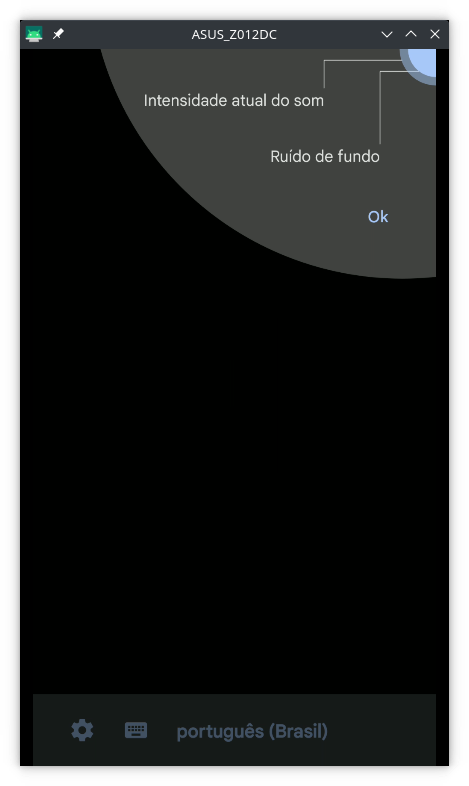
\includegraphics[width=\linewidth]{android_1.png}
    \caption{Ambiente do aplicativo para conversão de voz em texto - 1.}
    \label{fig:imagem1}
  \end{minipage}\hfill
  \begin{minipage}{0.45\textwidth}
    \centering
    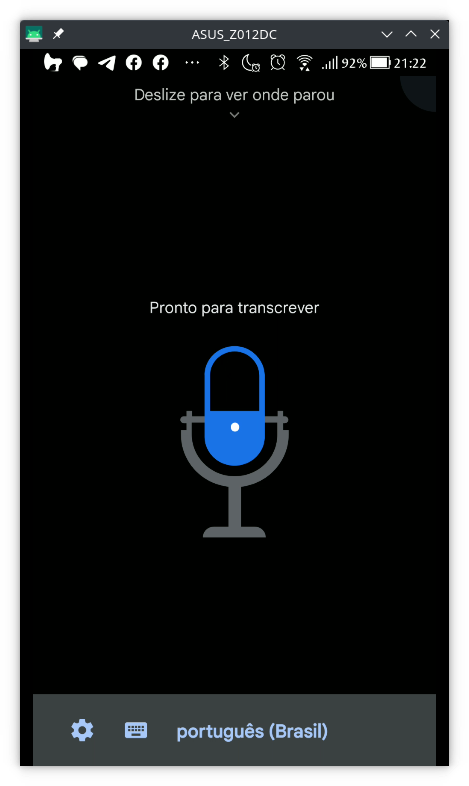
\includegraphics[width=\linewidth]{android_2.png}
    \caption{Ambiente do aplicativo para conversão de voz em texto - 2.}
    \label{fig:imagem2}
  \end{minipage}
  \vskip\floatsep
  \begin{minipage}{0.29\textwidth}
    \centering
    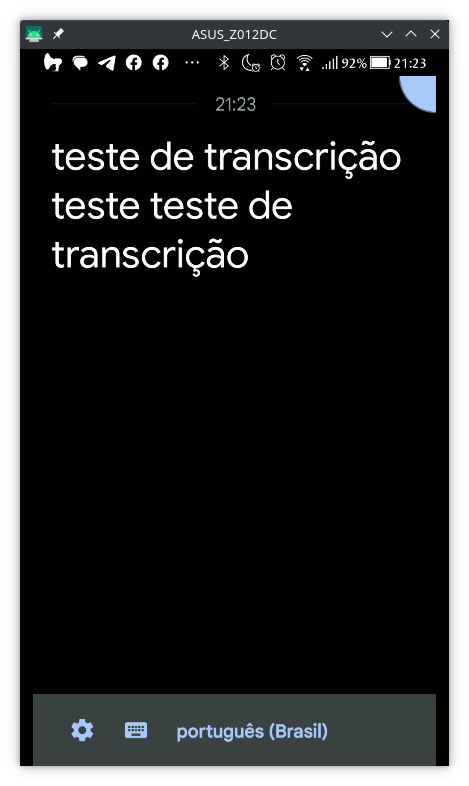
\includegraphics[width=\linewidth]{android_3.png}
    \caption{Teste do aplicativo para conversão de voz em texto.}
    \label{fig:imagem3}
  \end{minipage}\hfill
  \begin{minipage}{0.29\textwidth}
    \centering
    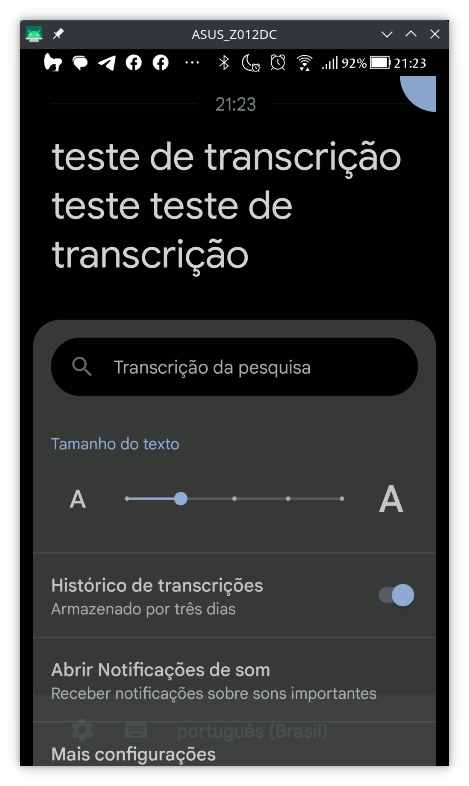
\includegraphics[width=\linewidth]{android_4.png}
    \caption{Configuração do aplicativo para conversão de voz em texto - 1}
    \label{fig:imagem4}
  \end{minipage}\hfill
  \begin{minipage}{0.29\textwidth}
    \centering
    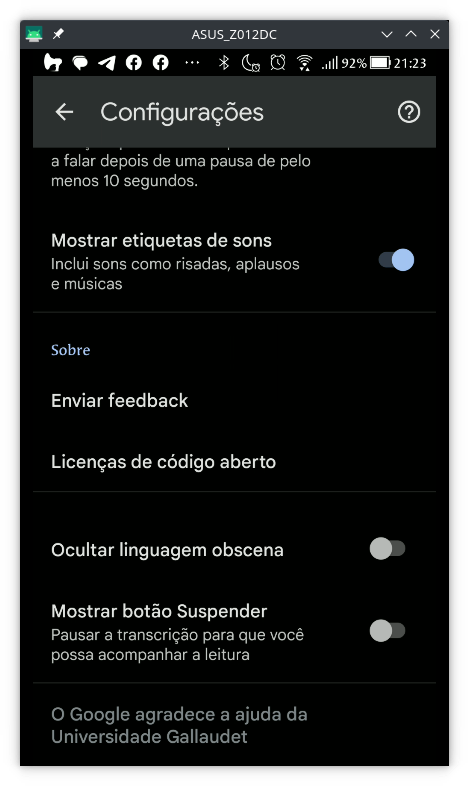
\includegraphics[width=\linewidth]{android_5.png}
    \caption{Configuração do aplicativo para conversão de voz em texto - 2}
    \label{fig:imagem5}
  \end{minipage}
\end{figure*}


Usando desta ferramenta, pode-se construir um corpus de texto, o qual será salvo no formato de arquivo .txt e usando da formatação UTF-8. Este corpus deve possuir tamanho significante sobre o qual pode-se medir a indexação e frequência de cada termo, devendo incluir várias entrevistas cada qual separada pelo marcador sequencial \verb|NUM_ENTRE_1|. Para tanto, deve-se pedir que os discentes entrevistados respondam às questões acerca do tema, e registrar cada resposta. Os agregados de resposta podem gerar arquivos de corpus de texto específicos divididos por seriação, idade, gênero ou outros recortes.



\section{Da contagem de frequências e indexação}

Estes procedimentos quantitativos\footnote{\citeonline{santos2021visao}} visam complementar a parte conceitual e qualitativa apresentada anteriormente, configuração que enquadra a pesquisa na abordagem quali-quanti. 

Eventuais coocorrências e associações da terminologia dotadas de significante correlação estatística\footnote{\citeonline{lexical_frequencies}} podem ser analisadas utilizando-se de ferramentas de linguística computacional, nomeadamente a biblioteca NLTK - Natural language toolkit\footnote{\citeonline{Python_NLTK}}, presente na linguagem Python 3.  Análises similares podem ser realizadas usando o software Iramutek. Acerca de tais técnicas vide \citeonline{klamt2021} e \citeonline{IRAMUTEQ_TUTORIAL}.

Os procedimentos quantitativos se iniciam com a importação do corpus para o ambiente da linguagem python 3. O documento corpus.txt deve conter as entrevistas transcritas usando a ferramenta de transcrição discutida acima e deve estar na mesma pasta onde o ambiente de trabalho do. A importação do arquivos selecionado para compor o corpus de texto pode ser realizada com a seguinte função na linguagem Python 3, apresentada no quadro \ref{importar}.



\begin{quadro}[htb]
\caption{Exemplo de código em Python 3 para importar um corpus e dividi-lo em entrevistas.}
\lstinputlisting[, label={importar}]{ex_01.py}
\fonte{Elaboração própria.}
\end{quadro}


A identificação das entidades presentes no texto e a identificação do idioma usado no corpus podem ser realizados nesta etapa. O código seguinte recebe um texto, relativo à uma das entrevistas e retorna uma lista de entidades e uma variável contendo o idioma; vide quadro \ref{entidades}

\begin{quadro}[htb]
\caption{Exemplo de código em Python 3 para identificar o idioma e as entidades num texto.}
\lstinputlisting[, label={entidades}]{ex_02.py}
\fonte{Elaboração própria.}
\end{quadro}


A limpeza do texto coletado é necessária afim de se eliminar stopwords e pontuação. Esta pode ser realizada nesta etapa, código à seguir, em  recebe um texto não processado e o idioma do mesmo, inferido pela função anterior e elimina as stopwords, pontuações e numeração; por fim retorna o texto limpo, o texto não processado, bigramas, trigramas, hapaxes; vide quadro \ref{limpar}


\begin{quadro}[htb]
\caption{Exemplo de código em Python 3 para limpar corpus de texto.}
\lstinputlisting[label={limpar}]{ex_03.py}
\fonte{Elaboração própria.}
\end{quadro}


O procedimento de cálculo de frequência e indexação que gera a OME pode ser realizado com o código presente no quadro \ref{ome}, o qual recebe o texto limpo e retorna uma lista das palavras ordenadas segundo OME e uma segunda lista de tuplas contendo o termo associado à sua respectiva OME.


\begin{quadro}[htb]
\caption{Exemplo de código em Python 3 para calcular os OME num corpus de texto.}
\lstinputlisting[label={ome}]{ex_04.py}
\fonte{Elaboração própria.}
\end{quadro}


\begin{figure}[h]
  \centering
  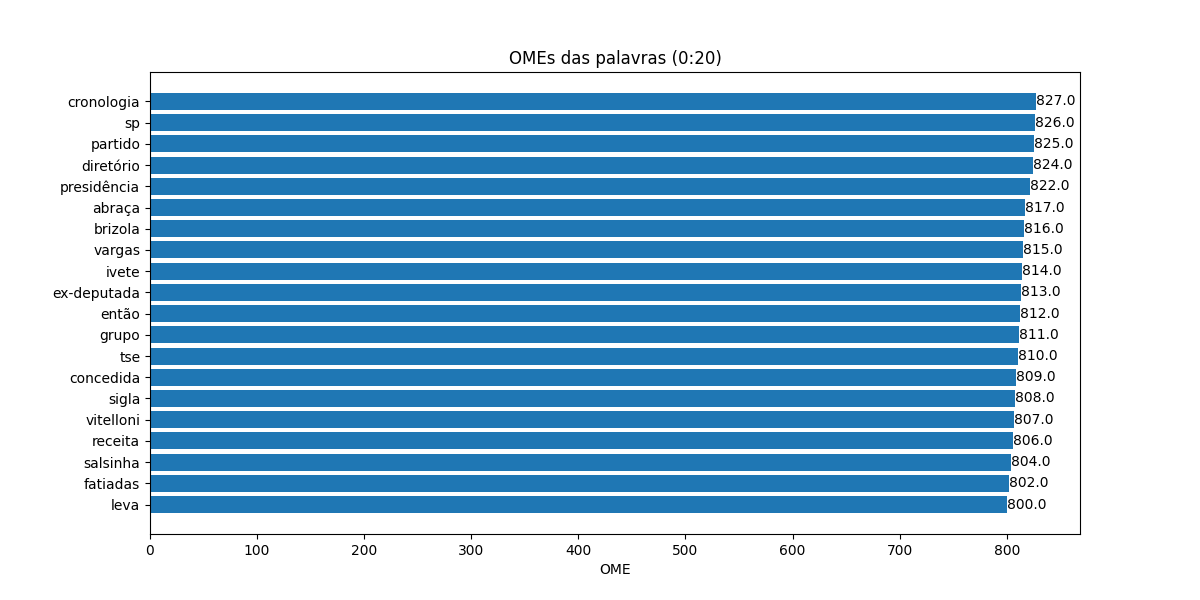
\includegraphics[width=0.8\textwidth]{OME_1.png}
  \caption{OME para os 10 primeiros elemento do corpus de teste.}
  \label{ome_0-10}
\end{figure}

A interpretação das frequências e a inferência dos elementos descrita por\citeonline{bardin_analise} permite o destaque dos elementos presentes no núcleo central, dos elementos intermediários e periféricos das RS. Tais representações de indexação e frequência podem ser apresentados usando a técnica do diagrama de Vergès\footnote{\citeonline[p.137]{representacoes_metodologia}} para se associar a frequência dos termos evocados à sua prioridade no discurso, contabilizando assim a OME\footnote{\citeonline{Evocacao_livre}}. Estes procedimentos podes ser realizados usando o código do quadro \ref{verges}, o qual recebe a lista das OMEs e as lista de palavras associadas as OMEs e retorna uma lista de tuplas contendo os elementos do núcleo central, e das zonas periférica 1, 2 e 3.


\begin{quadro}[htb]
\caption{Exemplo de código em Python 3 o qual parte das OME num corpus de texto e retorna o núcleo central, e as zonas periféricas.}
\lstinputlisting[label={verges}]{ex_05.py}
\fonte{Elaboração própria.}
\end{quadro}



\section{Do locus da coleta de dados}

Tais procedimentos de coleta de dados serão realizados pelo pesquisador no espaço do Colégio Instituto Estadual de Educação de Maringá, durante o período do segundo semestre do ano de 2022. Para o procedimento de coleta de dados será utilizado um questionário aberto seguido de entrevista transcrita afim de se produzir o corpus de texto analisado. Serão questionados os estudantes, de maneira voluntária, anônima e não-avaliativa, discentes nos 1\textordmasculine, 2\textordmasculine e 3\textordmasculine anos do NEM regular e técnico, uma vez que estes, devido à transição para a nova grade curricular, já foram expostos à temas adjacentes ao conteúdo das representações estudadas nas matérias de física, química e biologia. 




\section{Questionário e coleta de dados}

Serão questionados os estudantes, de maneira voluntária, anônima e não-avaliativa, discentes nos 1\textordmasculine, 2\textordmasculine e 3\textordmasculine anos do NEM regular e técnico, uma vez que estes, devido à transição para a nova grade curricular, já foram expostos à temas adjacentes ao conteúdo das representações estudadas nas matérias de física, química e biologia. 



\chapter{Produto educacional}

A produção de materiais didáticos acerca deste paradigma tecnológico se apresenta como necessária, visto que o tema traz diversos elementos interdisciplinares.

O produto educacional\footnote{Acerca do tema vide a contribuição de \citeonline{PRODUTOS_EDUCACIONAIS}} proposto será apresentado na forma de sequência pedagógica interdisciplinar contento elementos dos itinerários formativo do NEM\footnote{\citeonline{Itinirarios_nem}}. Tais conteúdos se apresentam nos itinerários de 'Ciências da Natureza e suas tecnologias' e de 'Ciências Humanas e Sociais aplicadas'. O produto pretende sanar as lacunas nas representações que forem percebidas no entendimento da problemática proposta, considerando-se aquilo que será inquirido aos discentes.

No itinerário de Ciências Humanas, tal conteúdo pode usar como argumento central uma linha do tempo histórica da transformações nas tecnológicas analisadas. Sugere-se que esta contextualização deve ser seguida da caracterização das práticas tecnológicas e da subsequente caracterização dos sistemas político-econômicos e suas consequências para o ambiente humano e natural. Por fim sugere-se que o material contenha uma análise de possíveis cenários futuros afim de reforçar a percepção da dinâmica de tais transformações. Possíveis tensões, críticas e outros elementos deletérios ou inviabilizadores da implementação de tais tecnologias podem ser incluídos afim de reforçar o detalhamento de tais transformações. Estão também presentes elementos das ciências humanas, na forma dos conceitos das disciplinas de filosofia e sociologia; nomeadamente: conceitos de paradigma, dialética, sistemas sociais e impacto humano sobre o meio ambiente.

Estão presentes elementos que pertencem ao itinerário das ciências da natureza, na forma dos conceitos das disciplinas de física e química; nomeadamente: conceitos de energia potencial, armazenada e gasta, energia cinética, química, térmica e nuclear, perda de energia, densidade energética, absorção e adsorção, termodinâmica, geração de eletricidade, consumo de eletricidade e sistemas industriais. Este produto pretende sanar a ausência de materiais educacionais acerca das tecnologias de armazenagem de energia, sua produção e consumo, e atende à necessidade de se criar comparações entre as diversas abordagens tecnológicas e suas respectivas densidades energéticas e impactos ambientais.

\section{Visualização dos dados}

O produto final também deve apresentar, associado às representações identificadas, elementos dos conteúdos reificados oriundos de materiais ainda não catalogados e sistematizados acerca do tema das formas de AE; fato sintomático da profusão de esforços de diversas organizações estatais, privadas e da sociedade civil organizada.

Prevê-se então que o produto educacional detalhará a historicidade concreta que permite a transição colocada por este paradigma tecnológico, característica que, como afirmado anteriormente, atende a necessidade de informar e subsidiar o processo de acompanhamento e avaliação vivenciado pela comunidade escolar e acadêmica, por agentes públicos e tomadores de decisão, impactados por tais mudanças tecnológicas e seus possíveis impactos.









\phantompart

\postextual
% ----------------------------------------------------------

% ----------------------------------------------------------
% Referências bibliográficas
% ----------------------------------------------------------
\bibliography{Interdisciplinaridade}

% ----------------------------------------------------------
% Glossário
% ----------------------------------------------------------
%
% Consulte o manual da classe abntex2 para orientações sobre o glossário.
%
%\glossary

% ----------------------------------------------------------
% Apêndices
% ----------------------------------------------------------

% ---
% Inicia os apêndices
% ---
%\begin{apendicesenv}

% Imprime uma página indicando o início dos apêndices
%\partapendices

% ----------------------------------------------------------
%\chapter{Quisque libero justo}
% ----------------------------------------------------------

%\lipsum[50]

% ----------------------------------------------------------
%\chapter{Nullam elementum urna vel imperdiet sodales elit ipsum pharetra ligula
% ac pretium ante justo a nulla curabitur tristique arcu eu metus}
% ----------------------------------------------------------
%\lipsum[55-57]

%\end{apendicesenv}
% ---


% ----------------------------------------------------------
% Anexos
% ----------------------------------------------------------

% ---
% Inicia os anexos
% ---
%\begin{anexosenv}

% Imprime uma página indicando o início dos anexos
%\partanexos

% ---
%\chapter{Morbi ultrices rutrum lorem.}
% ---
%\lipsum[30]

% ---
%\chapter{Cras non urna sed feugiat cum sociis natoque penatibus et magnis dis
% parturient montes nascetur ridiculus mus}
% ---

%\lipsum[31]

% ---
%\chapter{Fusce facilisis lacinia dui}
% ---

%\lipsum[32]

%\end{anexosenv}

%---------------------------------------------------------------------
% INDICE REMISSIVO
%---------------------------------------------------------------------
\phantompart
\printindex
%---------------------------------------------------------------------

\end{document}
